\documentclass[fontset=windows, 12pt]{article}
\PassOptionsToPackage{quiet}{fontspec}
\usepackage[a4paper, total={6.5in, 10in}]{geometry}
\usepackage{amsmath}
\usepackage{tikz}
\usepackage{ctex}
\usepackage{pgfplots}
\usepackage{tikz-3dplot}
\tdplotsetmaincoords{60}{110}
\pgfplotsset{compat=1.17}

\title{Use ChatGPT to Draw}
\author{Eureka}
\date{\today}

\begin{document}
\maketitle
\section{绘制普通正方体}
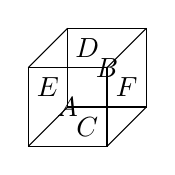
\begin{tikzpicture}[x=1cm, y=1cm, z=0.5cm]
    % Draw the cube
    \draw (0, 0, 0) -- (1, 0, 0) -- (1, 1, 0) -- (0, 1, 0) -- cycle;
    \draw (0, 0, 1) -- (1, 0, 1) -- (1, 1, 1) -- (0, 1, 1) -- cycle;
    \draw (0, 0, 0) -- (0, 0, 1);
    \draw (1, 0, 0) -- (1, 0, 1);
    \draw (1, 1, 0) -- (1, 1, 1);
    \draw (0, 1, 0) -- (0, 1, 1);

    % Labels
    \node at (0.5, 0.5, 0) {$A$};
    \node at (0.5, 0.5, 1) {$B$};
    \node at (0.5, 0, 0.5) {$C$};
    \node at (0.5, 1, 0.5) {$D$};
    \node at (0, 0.5, 0.5) {$E$};
    \node at (1, 0.5, 0.5) {$F$};
\end{tikzpicture}


\section{绘制边长为3实心正方体的LaTeX代码}
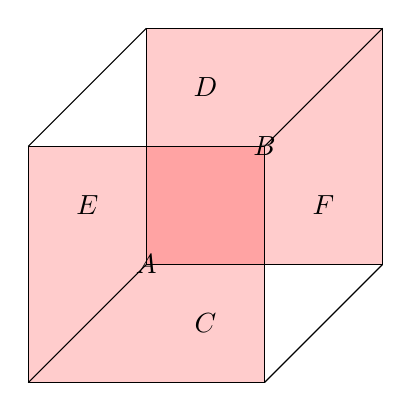
\begin{tikzpicture}[x=1cm, y=1cm, z=0.5cm]
    % Draw the cube
    \fill[red,opacity=0.2] (0, 0, 0) -- (3, 0, 0) -- (3, 3, 0) -- (0, 3, 0) -- cycle;
    \fill[red,opacity=0.2] (0, 0, 3) -- (3, 0, 3) -- (3, 3, 3) -- (0, 3, 3) -- cycle;
    \draw (0, 0, 0) -- (3, 0, 0) -- (3, 3, 0) -- (0, 3, 0) -- cycle;
    \draw (0, 0, 3) -- (3, 0, 3) -- (3, 3, 3) -- (0, 3, 3) -- cycle;
    \draw (0, 0, 0) -- (0, 0, 3);
    \draw (3, 0, 0) -- (3, 0, 3);
    \draw (3, 3, 0) -- (3, 3, 3);
    \draw (0, 3, 0) -- (0, 3, 3);

    % Labels
    \node at (1.5, 1.5, 0) {$A$};
    \node at (1.5, 1.5, 3) {$B$};
    \node at (1.5, 0, 1.5) {$C$};
    \node at (1.5, 3, 1.5) {$D$};
    \node at (0, 1.5, 1.5) {$E$};
    \node at (3, 1.5, 1.5) {$F$};
\end{tikzpicture}

\section{绘制一个三维坐标轴}
\begin{tikzpicture}[tdplot_main_coords, scale=3]
    % 绘制坐标轴
    \draw[thick,->] (-1,0,0) -- (1,0,0) node[anchor=north east]{$x$};
    \draw[thick,->] (0,-1,0) -- (0,1,0) node[anchor=north west]{$y$};
    \draw[thick,->] (0,0,-1) -- (0,0,1) node[anchor=south]{$z$};
\end{tikzpicture}


\section{绘制曼陀罗}
\begin{tikzpicture}[tdplot_main_coords, scale=3]
    % 定义坐标系的原点
    \coordinate (O) at (0,0,0);

    % 绘制第一个曼陀罗
    \draw[thick,red] (O) -- ++(0.5,0,0) arc (0:60:0.5 and 0.5);
    \draw[thick,red] (O) -- ++(0.5,{0.5*sqrt(3)},0) arc (0:60:0.5 and 0.5);
    \draw[thick,red] (O) -- ++(1,0,0);

    % 绘制第二个曼陀罗
    \draw[thick,blue] (O) -- ++(0.5,0,0) arc (0:-60:0.5 and 0.5);
    \draw[thick,blue] (O) -- ++(0.5,-{0.5*sqrt(3)},0) arc (0:-60:0.5 and 0.5);
    \draw[thick,blue] (O) -- ++(1,0,0);

    % 绘制第三个曼陀罗
    \draw[thick,green] (O) -- ++(0.5,0,0) arc (0:60:0.5 and 0.5);
    \draw[thick,green] (O) -- ++(0.5,{0.5*sqrt(3)},0) arc (0:60:0.5 and 0.5);
    \draw[thick,green] (O) -- ++(0.5,{0.5*sqrt(3)},0.5);

    % 绘制第四个曼陀罗
    \draw[thick,orange] (O) -- ++(0.5,0,0) arc (0:-60:0.5 and 0.5);
    \draw[thick,orange] (O) -- ++(0.5,{-0.5*sqrt(3)},0) arc (0:-60:0.5 and 0.5);
    \draw[thick,orange] (O) -- ++(0.5,{-0.5*sqrt(3)},0.5);
\end{tikzpicture}


\end{document}
